\subsection{Parking Lot Generation}
The ParkingGenerator is implemented as a function that takes a plot and its underlying terrain as input and produces a parking lot as output (see Table~\ref{table:parking}).
This generator in particular is responsible for filling roughly ten percent of the generated cities with parking lots, a percentage based on research conducted in Phoenix,~AZ~\cite{parking_percent}.
\begin{table}[H]
   \centering
   \begin{tabular}{lllll}
     \textbf{Input}                           &               & \textbf{Function}            &               & \textbf{Output}         \\
     \midrule
     \textit{Plot, Terrain}                   & $\rightarrow$ & \textbf{ParkingGenerator}       & $\rightarrow$ & \textit{Parking lot}           \\
     \bottomrule
   \end{tabular}

   \caption{Definition of the ParkingGenerator function which is responsible for generating parking lots.}
   \label{table:parking}
 \end{table}
 \vspace{-0.4cm}

One considered approach for generating parking lots was Esri CityEngine's \cite{Esri}.  % having a hard time finding this source, Anton who found it... plz help me. 
What they use, for at least some of their generation is simply covering areas with textures. This can be seen in their parks and parking lots. 
This was at first considered to be a viable option for the project, only it was found that it offers little alternatives for modification.

Modification, in this remark, includes the shape of the entire parking lot as well as the size of the individual parking spaces.
As every other generator provides fully scalable content, it would be inconvenient for the ParkingGenerator to be any different.
By using a single mesh with one texture applied to it, it would remove the possibility of scaling the size of the parking spaces within the mesh without scaling the mesh itself, which is not an option.

Another approach that we considered was to generate each line in the parking area individually which combines together to form multiple parking lots.
This was the initial approach that was used in the application, but due to performance concerns when dealing with multiple line objects, this had to be changed.

The final approach was a combination of the Esri method, and the method which had been previously used. 
The first step of this approach is to fill the plot with asphalt, but this is not an easy task as the mesh that is projected has to be perfectly aligned with the terrain mesh.
In order to avoid clipping issues, the algorithm basically cuts out a portion of the terrain in the shape of the plot, and then slightly offsets it upwards.
This means the mesh will never clip with the terrain, because it is based on the terrain mesh.

After that, the second step is to use a function for approximating the largest rectangle inside a polygon to find a suitable rectangle in the plot to generate parking lots in.
Based on the size of the approximated rectangle, the algorithm then generates multiple rows of parking lot.
Each row contains a quad that is projected onto the terrain with a transparent texture with only the white parking lot lines in it.
By modifying the UV coordinates of the quad, the texture can be repeated and scaled to the right size.
The plot is also given a certain margin around it to make sure there is enough space around the parking lots for cars to get in and out of the parking area.

The reasoning behind this algorithm was the group's observation that parking lots seem to have a rectangular shape generally (see Figure~\ref{fig:parkings}).
This shape does of course not apply to every parking lot in the world, however attempting to create parking lots of any size and shape would require a lot more effort, and was therefore deemed out of scope for this project. 

\begin{figure}[H]
  \centering
  \begin{subfigure}[b]{0.55\textwidth}
    \frame{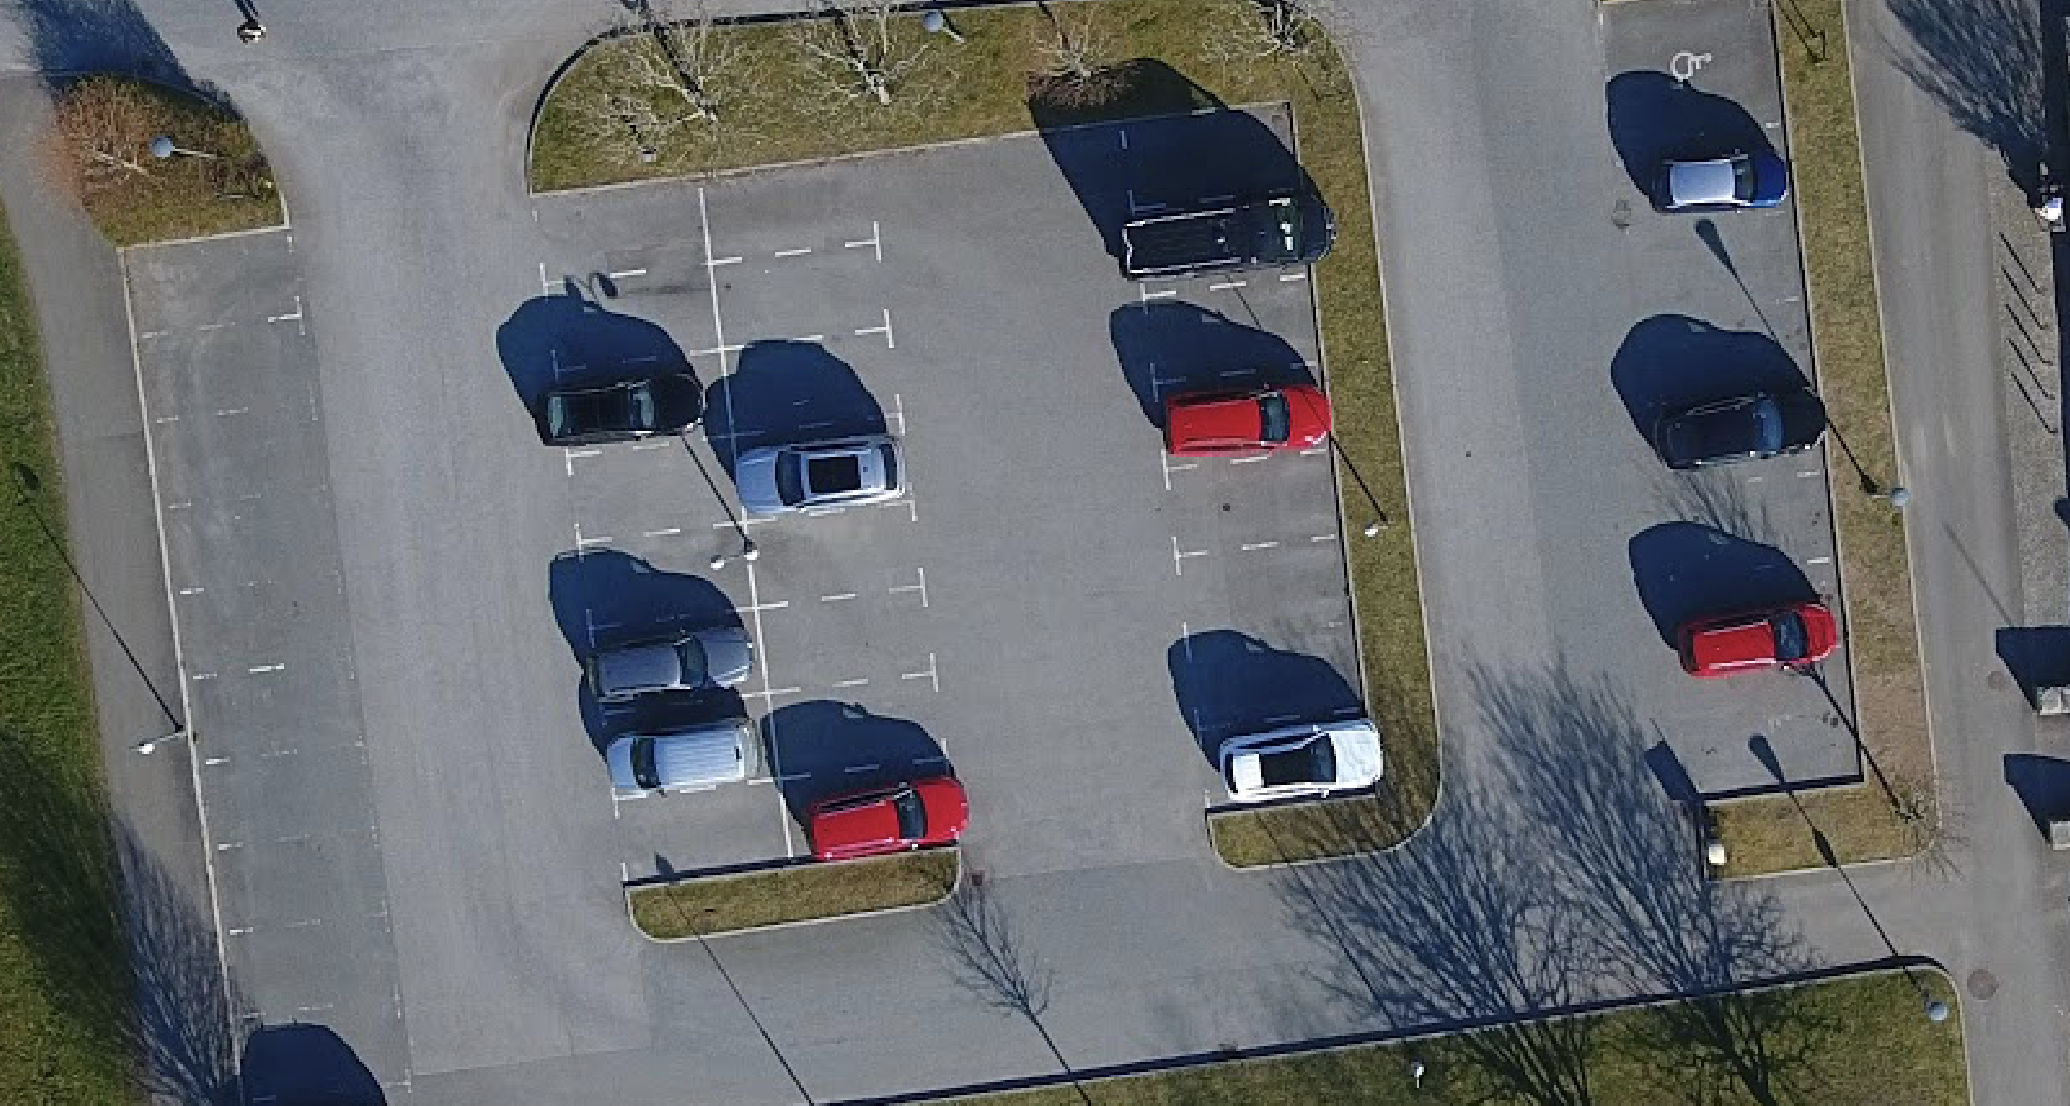
\includegraphics[width=\textwidth]{figure/parking1}}
  \end{subfigure}
  \quad
  \begin{subfigure}[b]{0.395\textwidth}
    \frame{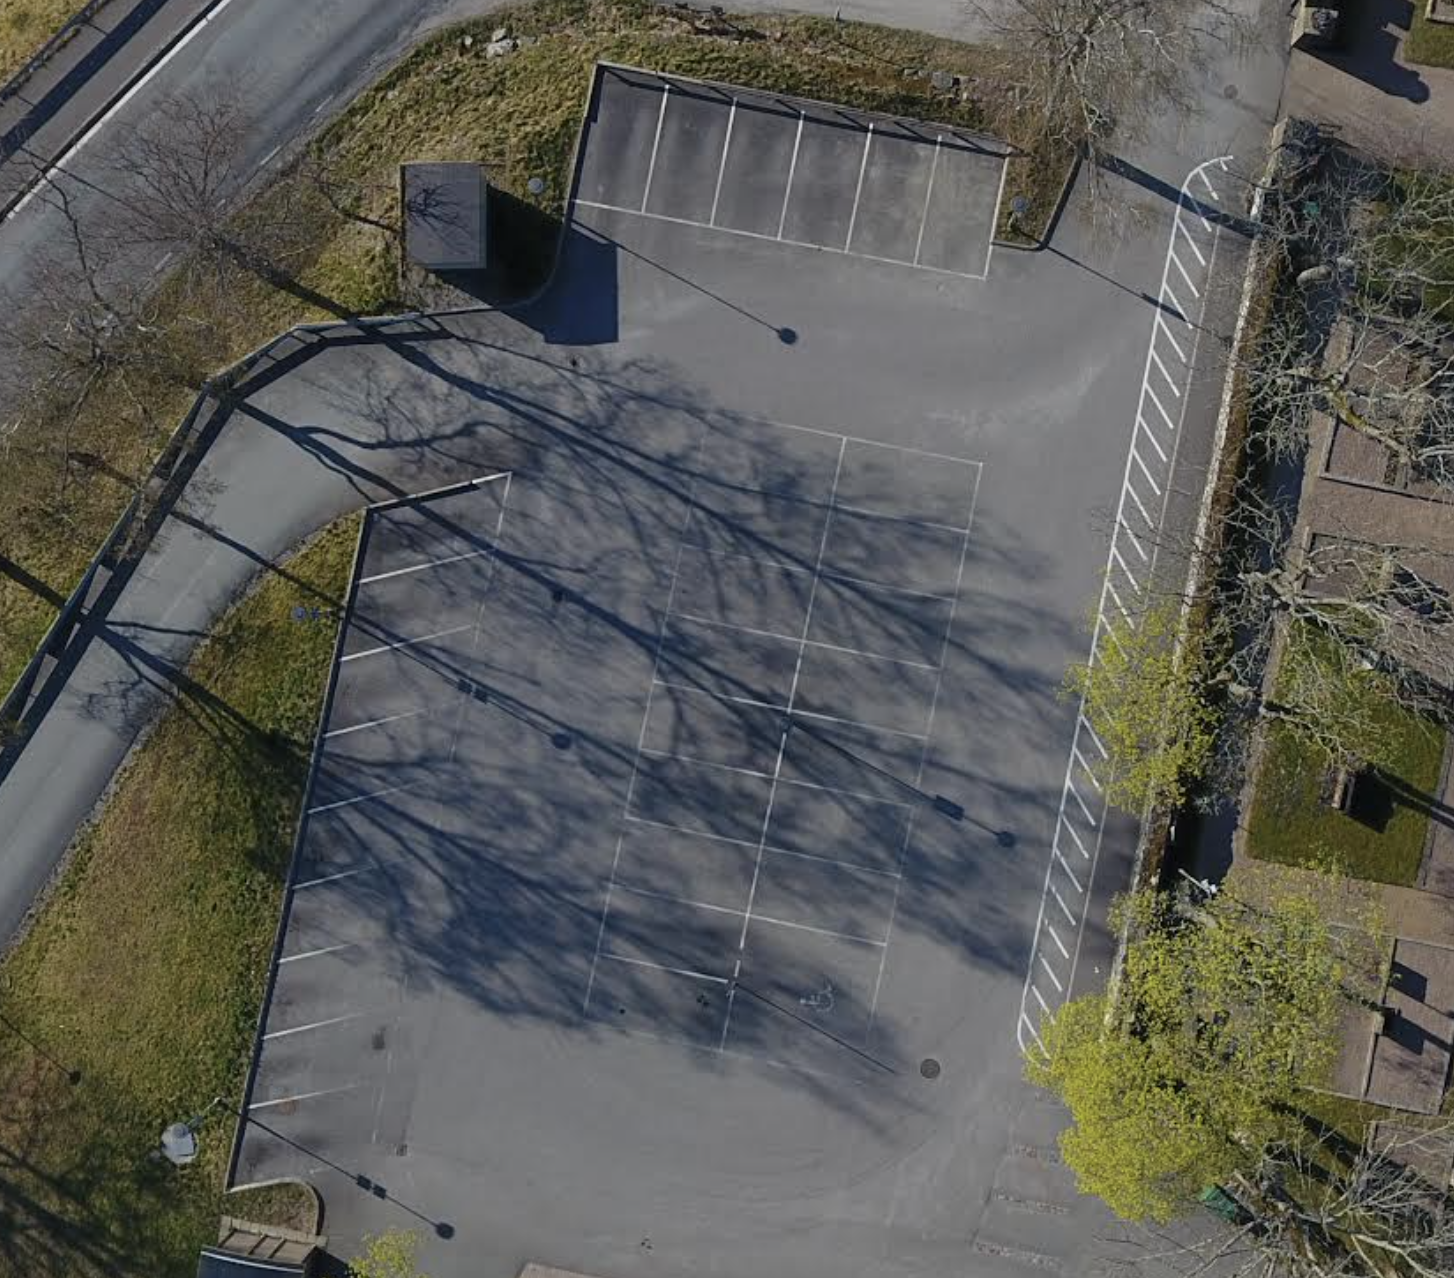
\includegraphics[width=\textwidth]{figure/parking2}}
  \end{subfigure}
  \caption{Two examples of parking lots observed by the project group, showcasing the rectangular shapes mentioned above.}
  \label{fig:parkings}
\end{figure}

\begin{figure}[H]
  \centering
  \begin{subfigure}[b]{0.485\textwidth}
    \frame{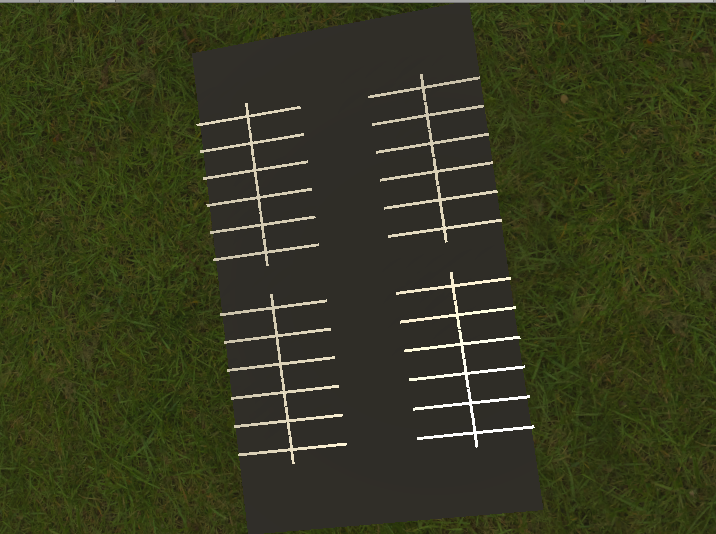
\includegraphics[width=\textwidth]{figure/fourcol}}
    \caption{Large parking lot consisting of four columns.}
  \end{subfigure}
  \quad
  \begin{subfigure}[b]{0.45\textwidth}
    \frame{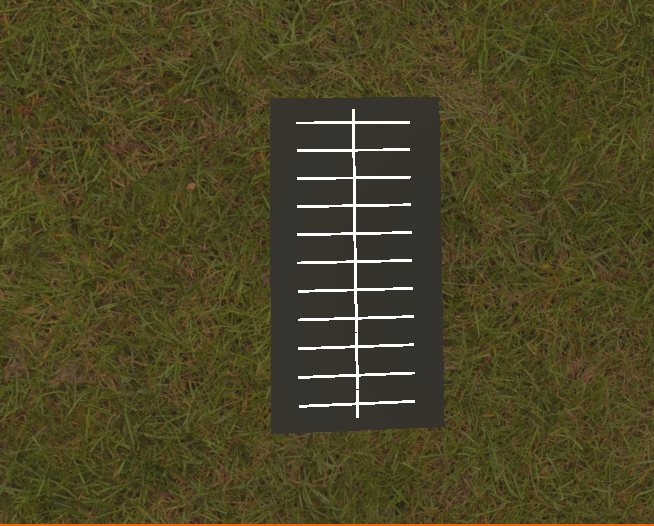
\includegraphics[width=\textwidth]{figure/twocol}}
    \caption{Small parking lot consisting of two columns.}
  \end{subfigure}
    \caption{Two examples of different sized parking lots created by the generator.}
  \label{fig:sizebased}
\end{figure}
